% -*- coding: utf-8; ispell-dictionary: "french"; -*-

%----------------------------
% Chapter 1 - Fragment Scade
%----------------------------


Scade a été développé par le laboratoire Verimag à partir des travaux sur
le langage synchrone Lustre, puis repris par Esterel-technologie. On retrouve
ainsi les notions de Lustre dans le langage de Scade, un programme est découpé
en noeuds dont les entrées et sorties sont des flux de données. Ces
noeuds sont les composants que nous voulons traduire. 
Les noeuds Scade considérés dans le cadre du projet $Cercles^2$ sont
soumis à quelques restrictions. En effet, il faut limiter le langage
utilisé, car certains éléments du langage sont spécifiques aux
langages synchrones et ne sont donc pas traduisibles en B.\\

% SECTION 1 : Présentation

\section{Architecture d'un composant Scade}

\paragraph{}
Scade étant un environnement de programmation par schémas-blocs, on
développe avec des boîtes. Par exemple, un programme d'addition sur deux flux d'entiers A
et B ayant pour sortie un flux C s'écrit:

\begin{figure}[h]
\begin{center}
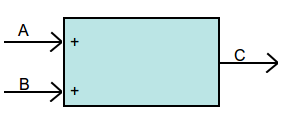
\includegraphics[scale=0.54]{1_add.png}
\end{center}
\caption{Schéma-block de l'addition}
\end{figure}

Ce langage en boîtes est basé sur le langage synchrone Lustre, et
c'est le programme en Lustre que nous allons parser avec le
traducteur. La représentation graphique du programme est ainsi
écrite en Lustre avant d'être traduite. C'est donc du code Lustre
que l'on traduit.

\begin{verbatim}
node ADD (A:int, B:int) returns (C:int);
let 
    C = A+B;
tel
\end{verbatim}


\paragraph{}
Les composants que nous voulons traduire sont formés d'un unique
noeud, dont la définition contient autant d'entrée et de sorties que
nécessaire. Il n'y a pas non plus de restriction sur le nombre de
variables locales utilisables.\\
Au niveau des types de données utilisées, on pourra manipuler
des entiers, réels et booléens. Et on pourra également manipuler des
tableaux de ces types. En revanche, les types définis par
l'utilisateur tels que les types enregistrement ne seront pas gérés
par le traducteur.\\
Le comportement du noeud est ensuite défini par une liste d'équations,
dont l'ordre n'a pas d'importance. Ces équations sont de la forme:
\begin{verbatim}
left_part = expr;
\end{verbatim}
Où left\_part désigne une variable locale ou une sortie du composant, et expr
est une expression portant sur une ou plusieurs variables locales ou entrées.

\paragraph{}
Les expressions disponibles sont toutes les expressions arithmétiques
(+, -, /, *, mod), les expressions relationnelles (<, >, <=, >=, =, <>)
et logiques (and, or, xor, not). Les expressions conditionelles sont également
possibles (if .. then .. else ..). On peut également faire des appels à d'autres
noeuds, sous condition qu'ils aient été traduits auparavant. \\
Sont également disponibles les opérations sur les tableaux, telles que
la définition, l'index, et la concaténation.\\


% SECTION 2 : Restrictions

\section{Restrictions}

\subsection{Le temps avec Scade}

Le temps est un élément primordial dans ces systèmes dits réactifs, où
on manipule des flux de données. Le temps est discrêtisé en instants,
et chaque instant correspond à 1 tic de l'horloge de base. A chaque
instant i, les équations du noeud sont résolues à partir du flux reçu
en entrée à cet instant, et produit le flux de sortie correspondant au
résultat.

\paragraph{Une horloge unique}
Ainsi, la première restriction à noter est qu'il n'y a qu'une seule
horloge, celle de base. Avec les langages synchrones, on peut
synchroniser des instructions sur des horloges différentes avec, mais
dans les programmes que nous manipulerons, il n'y aura donc pas de
définitions d'horloges, d'utilisation de when, ou current. Les
instructions d'un noeud sont toutes calculées sur l'horloge de base
uniquement. 

\paragraph{Des registres}
La seconde restriction concerne l'utilisation des opérateurs pre et
->. Ce sont des opérateurs temporels:
\begin{itemize}
\item pre X donne la valeur de l'expression X à l'instant précédent. A
l'instant 0 \footnote{On suppose que le premier instant est l'instant
0}, la valeur de pre X n'est pas définie. 
\item A -> B donne au premier instant la valeur de l'expression A, 
puis la valeur de l'expression B pour les instants allant de 1 à n. 
\end{itemize}
On ne pourra utiliser que la construction suivante utilisant ces deux
opérateurs: 
\begin{center}
$A\rightarrow(pre~X)$
\end{center}
Cette construction correspond au bloc SIMULINK 1/Z\footnote{Simulink MathWorks}, où A représente un
flux constant qui donnera la valeur de sortie à l'instant 0 du
bloc. Puis pour les instants 1 à n, on aura la valeur de l'expression
X à l'instant (1 à n)-1. \\
On appellera cette construction un registre, qui est initialisé avec la
valeur A, et qui permet d'accéder à la valeur précédente de X à tout
instant. Cette construction permet de donner un état à un composant.


\subsection{Contrats}

\paragraph{Assertions}
On peut définir des assertions dans un noeud afin de poser des
restrictions sur les valeurs d'entrée ou de sortie du composant. Avec
Scade, ces assertions sont possibles avec :
\begin{itemize}
\item \emph{assume x: expr}, où x est une des entrées du noeud, et
expr un prédicat portant sur cette entrée.
\item \emph{guarrantee x: expr}, où x est une des sorties du noeud, et
expr un prédicat portant sur cette sortie.
\end{itemize}
Ces assertions forment le contrat du composant, et seront
obligatoires sauf pour la restriction sur les booléen qui est triviale (la
valeur sera vraie ou fausse).\\
Par exemple, en reprenant le noeud ADD précédent, on impose comme condition sur
les entrées qu'elles doivent être comprises entre 0 et 100 inclus. Si les
préconditions sont respectées, alors la sortie sera comprise entre 0 et 200 inclus:
\begin{verbatim}
node ADD (A:int, B:int) returns (C:int);
let 
    assume A : A <= 100 & A >= 0;
    assume B : B <= 100 & B >= 0;
    guarantee C : C <= 200 & C >= 0;
    C = A+B;
tel
\end{verbatim}

